\thispagestyle{fancy}
\chapter{System Architecture} \label{ch:system_architecture}
\section*{\centering Chapter \thechapter}
\section*{\centering System Architecture}

The trainer module is responsible for generating and training supervised learning models. This module sends trained models to the selection module for performance evaluation. The selection module generates performance files and ranks the models according to its performance with respect to parameters if sent by the user. Rank obtained by model is used for selection of the best model. This best model is stored for future predictions. This model can be accessed by the prediction module. This module takes a user provided dataset and makes predictions with help of the best model. \Cref{fig:system_architecture} shows the whole process.

\begin{figure}[H]
  \centering
  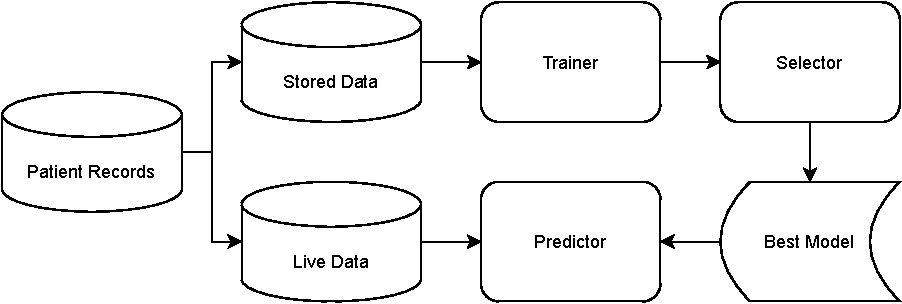
\includegraphics[width=0.7\columnwidth]{media/architecture/System Architecture.pdf}
  \caption{System architecture}
  \label{fig:system_architecture}
\end{figure}

\section{Data Flow in system}

The data used in this process goes through this sequential process shown in \cref{fig:data_flow_in_system}

\begin{figure}[H]
  \centering
  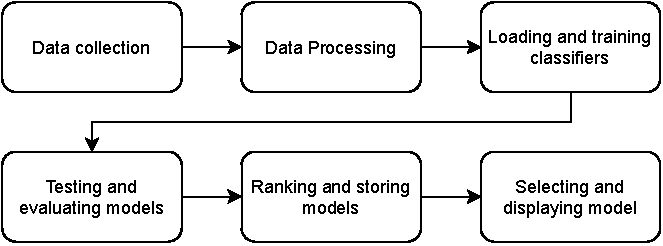
\includegraphics[width=0.7\columnwidth]{media/website/architecture/Data_Flow_System.pdf}
  \caption{Training and Selection Process}
  \label{fig:data_flow_in_system}
\end{figure}

\textbf{Data collection:} Collection of data is the first step in this process. The data is collected from the user. The data is stored in a local directory for further processing. The data is then divided into training and testing sets.

\vspace{-0.5em}
\textbf{Data processing:} In this step data labels are converted to 1 or 0, with respect to previous values. In case of data with more than 2 labels, labels with min value are converted to 0 and other values are converted into 1.

\vspace{-0.5em}
\textbf{Loading and training classifiers:} In this step model templates are used for generation of models. These models are trained with the help of processed training data.

\vspace{-0.5em}
\textbf{Testing and evaluating models:} The trained models are evaluated with help of processed testing datasets. The performance metrics are stored for ranking models.

\vspace{-0.5em}
\textbf{Ranking and storing models:} Performance metrics obtained in previous steps are used to rank the models, the models are stored in a local directory.

\vspace{-0.5em}
\textbf{Selecting and displaying model:} In this step rank of models are used for selection of best model, this model is stored into best models directory for future predictions. The name of this selected model is displayed to the user.

\section{Training and selection process} \label{sec:data_flow}

As shown in \cref{fig:training_and_selection_process}, the system is provided with a dataset, in this case records of ECG reports of patients. This data is already provided with labels. These labels can be boolean values i.e., 1 for True, and 0 for False, or they can have a series of values starting from 0. This data is further divided into training dataset and testing dataset. These datasets are forwarded to the extraction process. In the extraction process, datasets labels are converted into 0 and 1, this will eliminate extra classes present in labels by changing their value to 1. The processed training dataset is sent for the model training. As soon as this process takes place, the training module accesses premade models templates, and generates the model for training purposes. These models are trained with processed training data and stored in a directory for evaluation purposes.

\begin{figure}[H]
  \centering
  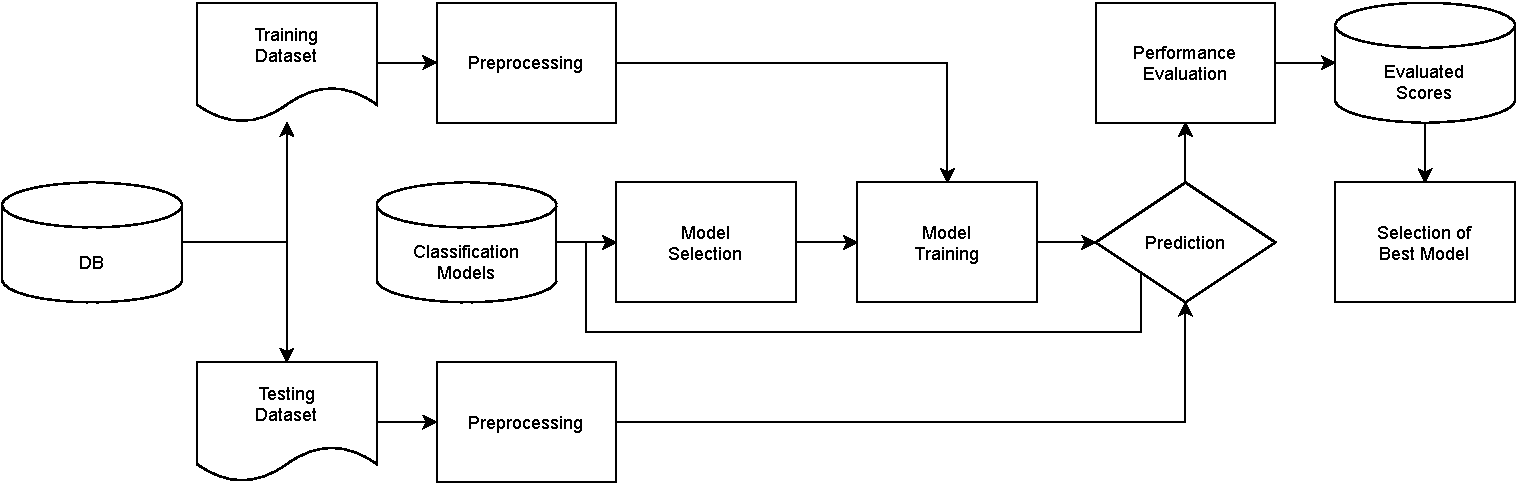
\includegraphics[width=0.9\columnwidth]{media/architecture/Process.pdf}
  \caption{Training and Selection Process}
  \label{fig:training_and_selection_process}
\end{figure}

Selector module accesses the stored models and processed testing dataset to evaluate the performance of models. The performance metrics used for evaluation are accuracy score, F1 score, precision score, recall score, roc score and prediction time of model. These parameters are multiplied with default or user provided weightage provided to generate scores of the models. These scores are stored and used to select the best suited model.

\section{Methodology}\label{sec:methodology}

\Cref{fig:model_selection_approach} shows the approach to the selection of a suitable model. The system can handle an infinite number of models. For each model, six performance parameters are used. These performance metrics are accuracy P$_1$, F1 score P$_2$, precision P$_3$, recall P$_4$, area under the ROC P$_5$, and prediction time P$_6$. From these, the first five parameters are grouped and given a weightage range between 0.2 and 1.0, whereas prediction time is given a weightage range between 0.25 to 0.75. \Cref{eq:v_score} shows the mathematical formula used to calculate the Vscore of the models.

For models M$_1$, M$_2$,..., M$_n$, the Vscores V$_1$, V$_2$,..., V$_n$ are obtained. These obtained Vscores are compared with each other. The model with the highest Vscore is selected as the most-suited model.

\begin{equation}\label{eq:v_score}
    V_{score} = \left(\sum_{x=1}^{5} w_xP_x\right) - w_6^2P6
\end{equation}

\begin{itemize}
    \item[where,]
    \item[$V_{score}$] Vscore of the model
    \item[$w_x$] The weightage generated by the system for the $x^{th}$ parameter.
    \item[$P_x$] Performance of $x^{th}$ parameter
\end{itemize}

\begin{figure}
  \centering
  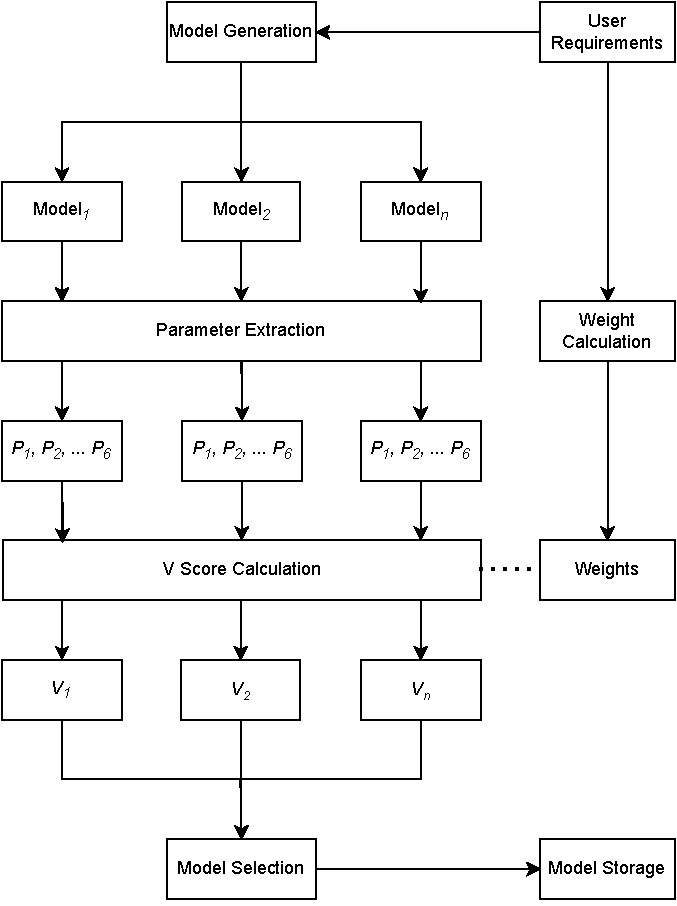
\includegraphics[width=0.9\columnwidth]{media/architecture/math_model_relaxed.pdf}
  \caption{Model Selection Approach}
  \label{fig:model_selection_approach}
\end{figure}

\section{Classifiers Used} \label{sec:supervised_learning}

The classifiers are algorithms that classify data into two or more classes based on rules set out by users. The models trained with these classifiers are used for classification purposes. In this project we are using classifiers to train models, these models will output data into two classes.

By default this system uses five different classifiers, they are K-Nearest Neighbors, Decision Tree, Random Forest, Multilayer Perceptron and Support vector machines. These classifiers are categorized as supervised learning algorithms or classifiers. These classifiers will predict the classes of data provided by the user.

\subsection{K-Nearest Neighbors} \label{subsec:K_nearest_neighbors}

K-nearest neighbor (KNN) algorithm is a supervised machine learning algorithm. Classification and regression problems such as multiclass problems are solved using this algorithm. KNN is lazy learning and non-parametric algorithm, which can be advantages or disadvantages depending on the user's requirements. These properties make this algorithm very effective and uncomplicated in general tasks. The drawback of the simplicity is the slow prediction time.

\subsubsection{Algorithm for K-Nearest Neighbors:}
\begin{steps}
  \vspace{-0.5em}
  \setlength{\itemsep}{-0.2em}
  \item Determine the number of K neighbors.
  \item Determine the Euclidean distance between the K neighbors.
  \item Using the estimated Euclidean distance, find the K nearest neighbors.
  \item Count the number of data points in each category among these K neighbors.
  \item Assign new data points to the category with the greatest number of neighbors.
  \item The model is now complete.
  \vspace{-1em}
\end{steps}

\subsection{Decision Tree} \label{subsec:decision_tree}
Decision trees are the most popular and effective tool for classification and prediction. The decision tree is a flow chart-like tree structure, where each internal node specifies a test for the attribute, each branch represents the result of the test, and each leaf node contains a class label. Decision trees are the most popular high-performance tool for classification and prediction.

\subsubsection{Construction of Decision Trees:}
\vspace{-0.5em}
The trees are trained by subdividing the features into subsets based on the attribute values. This process is run recursively on derived subsets. The recursion completes when all subsets of nodes have the same value for the target variable or if the split doesn't add any additional value to the prediction. Building a decision tree classifier is suitable for exploratory knowledge discovery as it does not require domain knowledge or parameter adjustment. Decision trees can handle high-dimensional data. In general, decision tree classifiers are more accurate. Decision tree induction is a typical inductive approach to learning classification knowledge.

\subsubsection{Alogrithm for Decision Trees:}
\begin{steps}
  \vspace{-0.5em}
  \setlength{\itemsep}{-0.2em}
  \item Start the tree on the root node that contains the complete dataset.
  \item Use the Attribute Selection Scale (ASM) to find the best attribute in the dataset.
  \item Divide S into a subset containing the possible values of the best attributes.
  \item Create a decision tree node with the best attributes.
  \item Recursively build a new decision tree using the subset of the dataset created in step 3. Continue this process until you reach a stage where you can no longer classify the node,   and you can call the last node a leaf node.
  \vspace{-1em}
\end{steps}

\subsection{Random Forest} \label{subsec:random_forest}
Random forest is a supervised learning algorithm based on a decision tree algorithm. This algorithm generates multiple decision trees from the provided sample. These decision trees are combined, and a majority vote is taken to solve the classification and regression problem. The Random Forest classifier offers more accurate and stable predictions at a slightly slower prediction time when compared with a decision tree.

\subsubsection{Bagging}
\vspace{-0.5em}
The random forest classifier is a type of ensemble classifier which uses the bagging technique. Random samples from data sets are collected. These samples generate independent models. Random forest uses decision tree classifiers for model generation. The final output is generated based on majority voting after combining the results of all models. This process of combination and majority voting is known as the aggregation process.

\subsubsection{Classification algorithm for Random Forest:}
\begin{steps}
  \vspace{-0.5em}
  \setlength{\itemsep}{-0.2em}
  \item N number of random records are taken from the dataset with k number of reports.
  \item Each sample generates a separate decision tree.
  \item Each decision tree will generate an output/prediction unrelated to other trees.
  \item The final output is determined based on majority voting in classification problems.
  \vspace{-1em}
\end{steps}

\subsection{Multi-layer Perceptron} \label{subsec:multi_layer_perceptron}
The multilayer perceptron is a neural network-based supervised learning algorithm. In this network, input and output are not linearly mapped. It is a feedforward algorithm hence more suitable for classification and regression problems. MLP uses a backpropagating algorithm for training, making it faster and usable for general predictions.

\subsubsection{Construction of MLP}
\vspace{-0.5em}
The neural network is made up of three primary components, neuron, activation function, and layers.

\vspace{-1em}
\textbf{Neuron:}
A neuron is the smallest unit of a neural network. It is based on neurons in the brain, which take one or more inputs to produce an output. The inputs are weighted, and each neuron has biases which are also weighted similar to inputs.

\vspace{-1em}
\textbf{Activation functions:}
The weighted sum of inputs and bias is passed through activation functions. This function serves as a mapping between two layers. These functions are usually non-linear. Activation functions control the firing of a neuron. We are using the sigmoid as an activation function. The sigmoid function returns either a zero or postitive value.

\vspace{-1em}
\textbf{Layers:}
Layers are rows of neurons in the network. The input layer is the entry point for the neural network. The output layer serves as the exit point for the neural network. A hidden layer or series of hidden layers connects input and output layers. In MLP, input layers take multiple
features as data. The output layer returns either 1 or 0.

\subsubsection{Algorithm for Multilayer Perceptron:}
\begin{steps}
  \vspace{-0.5em}
  \setlength{\itemsep}{-0.2em}
  \item N number of epochs is calculated by dividing sample size S by batch size B.
  \item Input layers accept the data features.
  \item Input layer forward data to hidden layers, which forward data to the output layer.
  \item Errors are calculated by comparing expected output and network output.
  \item The error propagated backward to adjust the weights of the network.
  \item All weights in the network are adjusted.
  \item Process in steps 3-6 is known as an epoch. The process is run for N number of epochs.
  \vspace{-1em}
\end{steps}

\vspace{-2em}
\subsection{Support Vector Machine} \label{subsec:support_vector_machine}
Support Vector Machines or SVM is one of the most commonly used supervised learning algorithms for data classification and regression. This algorithm is primarily used to solve classification problems in machine learning. The SVM algorithm created decision boundaries to divide n-dimensional spaces into classes. The new data points are categorized using these classes. The best boundary line which compartmentalizes most data accurately is called a hyperplane. The SVM algorithm uses vectors to create the hyperplane. Support vectors handle extreme cases giving the algorithm its name Support Vector Machine.

\vspace{-1em}
\textbf{Hyperplane:} A decision boundary separates new data points into different classes. The decision boundary that produces the most accurate categorization is called the hyperplane. The hyperplane adjusts with new data points by repositioning or introducing new dimensions. Hyperplanes can be linear or non-linear, depending on user requirements.

\vspace{-1em}
\textbf{Support Vectors:} These are extreme data points present in data sets. Support vectors have very close proximity to the hyperplane. Support vectors can directly affect the position and dimensions of the hyperplane.

\subsubsection{Tuning parameters of SVM}
\vspace{-0.5em}
Tuning parameters used in this projects are:

\vspace{-1em}
\textbf{Kernal:} SVM uses the kernel function to solve problems. These functions allow smoother operations on high dimensions. With kernels, SVM hyperplanes can theoretically reach infinite dimensions. Kernels also reduce complexity at higher dimensions. The primary purpose of the kernel is to provide a hyperplane way to accommodate non-linear datasets. In this project, we are providing an RBF kernel. This kernel is suitable for both small and large quantities of data.

\vspace{-1em}
\textbf{C parameter:} This is also known as the regularization parameter. C parameter suggests SVM optimization amount of margin used by a hyperplane. A higher value of the C parameter produces accurate results. Conversely, a lower value results in fast but less accurate predictions.

\vspace{-1em}
\textbf{Gamma:} The Gamma parameter defines the amount of influence of a model over the dataset. Gamma is inversely proportional to the curve of influence of the model. Lower gamma results in higher accuracy, but it is prone to overfitting. Higher gamma is constraining but can't handle complexity.

% \begin{figure}[H]
%     \centering
%     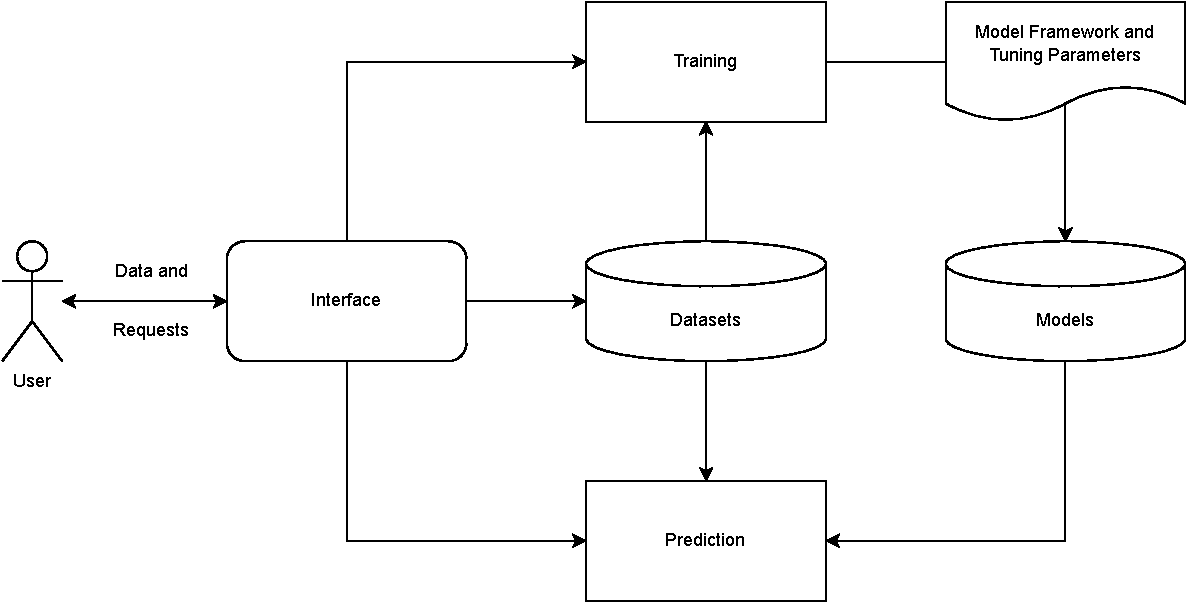
\includegraphics[width=0.9\columnwidth]{media/architecture/web_system_arch.pdf}
%     \caption{Web system architecture}
%     \label{fig:web_system_architecture}
% \end{figure}
